\chapter{Capitolo 22}
\section{Posta elettronica sicura e S/MIME}
\textbf{S/MIME} (Secure/Multipurpose Internet Mail Extension) è un miglioramento della sicurezza allo standard di formato di posta elettronica Internet MIME.
\subsection{MIME}
MIME è un'estensione del vecchio RFC 822 (Standard For The Format Of ARPA Internet Text Messages, 1982): la specifica di un formato di posta Internet. L'RFC 822 definisce una semplice intestazione con i campi "A", "Da", "Oggetto" e altri, che può essere utilizzata per instradare un messaggio di posta elettronica attraverso Internet e che fornisce informazioni di base sul contenuto dell'e-mail. RFC 822 presuppone un semplice formato di testo ASCII per il contenuto. 

\singlespacing

MIME fornisce una serie di nuovi campi di intestazione che definiscono le informazioni sul corpo del messaggio, tra cui la il corpo del messaggio, compreso il formato del corpo stesso. Soprattutto, MIME definisce una serie di formati di contenuto, che standardizzano le rappresentazioni formati di contenuto, che standardizzano le rappresentazioni per il supporto della posta elettronica multimediale. Gli esempi includono testo, immagini, audio e video.

\subsection{S/MIME}
S/MIME è una funzionalità complessa, definita in una serie di documenti. 

\singlespacing

I documenti più importanti relativi a S/MIME sono i seguenti:
\begin{itemize}
    \item \textbf{RFC 5750} (S/MIME Version 3.2 Certificate Handling, 2010)
    
    Specifica le convenzioni convenzioni per l'utilizzo dei certificati X.509 da parte di (S/MIME) v3.2.
    
    \item \textbf{RFC 5751} (S/MIME Version 3.2 Message Specification, 2010)
    
    Il principale documento di definizione per la creazione e l'elaborazione dei messaggi S/MIME.
    
    \item \textbf{RFC 4134} (Esempi di messaggi S/MIME, 2005)
    
    Fornisce esempi di messaggi formattati utilizzando S/MIME.
    
    \item \textbf{RFC 2634} (Enhanced Security Services for S/MIME, 1999)
    
    Descrive quattro estensioni opzionali dei servizi di sicurezza per S/MIME.
    
    \item \textbf{RFC 5652} (Sintassi crittografica dei messaggi (CMS), 2009)
    
    La sintassi crittografica è utilizzata per firmare digitalmente, digerire, autenticare o crittografare il contenuto di un messaggio contenuto di un messaggio.
    
    \item \textbf{RFC 3370} (Algoritmi CMS, 2002)
    
    Descrive le convenzioni per l'utilizzo di diversi algoritmi crittografici con il CMS.
    
    \item \textbf{RFC 5752} (Multiple Signatures in CMS, 2010)
    
    Descrive l'uso di firme multiple firme parallele per un messaggio.
    
    \item \textbf{RFC 1847} (Security Multiparts for MIME-Multipart/Signed and Multipart/ Encrypted, 1995)
    
    Definisce un quadro di riferimento all'interno del quale i servizi di sicurezza possono essere di sicurezza alle parti del corpo MIME. L'uso di una firma digitale è rilevante per S/MIME, come spiegato in seguito.
\end{itemize}

\begin{figure}[H]
	\centering
    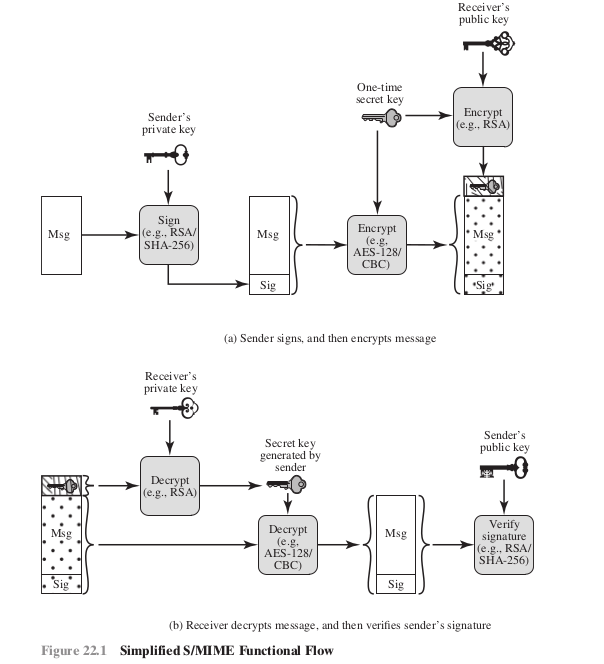
\includegraphics[width=14cm, keepaspectratio]{Bistarelli/img/cap_22/figura22.1.png}
\end{figure}

La funzionalità S/MIME è integrata nella maggior parte dei moderni software di posta elettronica e interoperano tra loro. S/MIME è definito come un insieme di tipi di contenuto MIME aggiuntivi (vedi Tabella 22.1).
(vedi Tabella 22.1) e fornisce la possibilità di firmare e/o crittografare i messaggi di posta elettronica. In sostanza, questi tipi di contenuto supportano quattro nuove funzioni:
\begin{itemize}
    \item \textbf{Dati criptati:} Consiste in contenuti criptati di qualsiasi tipo e chiavi di criptazione del contenuto criptato per uno o più tipi di messaggi di uno o più destinatari.
    
    \item \textbf{Dati firmati:} Una firma digitale si forma prendendo il message digest del contenuto da firmare, quindi crittografandolo con la chiave privata del firmatario. Il contenuto e la firma sono poi codificati con la codifica base64. Un messaggio di dati firmato può essere visualizzato solo da un destinatario con capacità S/MIME.
    
    \item \textbf{Dati con firma in chiaro:} Come per i dati firmati, viene creata una firma digitale del contenuto. Tuttavia, in questo caso, solo la firma digitale è codificata utilizzando base64. Di conseguenza, i destinatari senza capacità S/MIME possono visualizzare il messaggio, ma non possono verificare la firma.
    
    \item \textbf{Dati firmati e imbustati:} Le entità solo firmate e solo crittografate possono essere nidificate, quindi i dati crittografati possono essere firmati e i dati firmati o con firma in chiaro possono essere crittografati.
\end{itemize}

\paragraph{Dati firmati e firmati in chiaro} Gli algoritmi preferiti per la firma dei messaggi S/MIME utilizzano una firma RSA o un algoritmo di firma digitale (DSA) di un hash del messaggio SHA-256. Il processo funziona come segue. Si prende il messaggio che si vuole inviare e lo si mappa in un codice a lunghezza fissa di 256 bit, utilizzando SHA-256. Il digest del messaggio a 256 bit è, a tutti gli effetti, unico per questo messaggio. Quindi, S/MIME cripta il digest utilizzando RSA e la chiave privata RSA del mittente. Il risultato è la firma digitale, che viene allegata al messaggio. Ora, chiunque riceva il messaggio può ricalcolare il digest del messaggio e decifrare la firma usando RSA e la chiave pubblica RSA del mittente. Se il digest del messaggio nella firma corrisponde al digest del messaggio calcolato, la firma è valida. Poiché questa operazione comporta solo la crittografia e la decrittografia di un blocco di 256 bit, richiede poco tempo. Il DSA può essere utilizzato come algoritmo di firma al posto dell'RSA. La firma è una stringa binaria, e l'invio in questa forma attraverso il sistema di posta elettronica Internet potrebbe comportare un'alterazione involontaria del contenuto, perché alcuni software di posta elettronica tenteranno di interpretare il messaggio. Per proteggere i dati, la firma da sola o la firma più il messaggio vengono mappati in caratteri ASCII stampabili utilizzando uno schema noto come mappatura radix-64 o base64. Radix-64 mappa ogni gruppo di ingresso di tre ottetti di dati binari in quattro caratteri ASCII. di dati binari in quattro caratteri ASCII (vedi Appendice G).

\singlespacing

\paragraph{Dati criptati} Gli algoritmi predefiniti utilizzati per la crittografia dei messaggi S/MIME sono
AES e RSA. Per iniziare, S/MIME genera una chiave segreta pseudorandom. In qualsiasi applicazione di crittografia convenzionale, è necessario affrontare il problema della distribuzione della chiave. In S/MIME, ogni chiave convenzionale viene utilizzata una sola volta. Cioè, viene generata una nuova chiave pseudorandom per ogni nuova crittografia del messaggio. Questa chiave di sessione è legata al messaggio e trasmessa con esso. La chiave segreta viene utilizzata come input per l'algoritmo di crittografia a chiave pubblica RSA, che cripta la chiave con la chiave pubblica RSA del destinatario. Sul lato ricevente, S/MIME utilizza la chiave privata RSA del destinatario per recuperare la chiave segreta. e poi utilizza la chiave segreta e AES per recuperare il messaggio in chiaro. Se si utilizza solo la crittografia, si usa il radix-64 per convertire il testo cifrato in formato ASCII.

\singlespacing

\paragraph{Certificati a chiave pubblica} Come si può notare da quanto discusso finora, S/MIME contiene un insieme intelligente, efficiente e interconnesso di funzioni e formati per fornire un efficace servizio di crittografia e firma. Per completare il sistema, è necessario affrontare un'ultima area, quella della gestione delle chiavi pubbliche. Lo strumento di base che consente un uso diffuso di S/MIME è il certificato a chiave pubblica. S/MIME utilizza certificati conformi allo standard internazionale X.509v3.

\section{Domainkeys che identifica la posta}
DomainKeys Identified Mail (DKIM) è una specifica per la firma crittografica dei messaggi di posta elettronica, che consente a un dominio firmatario di rivendicare la responsabilità di un messaggio nel flusso di posta. I destinatari dei messaggi (o gli agenti che agiscono per loro conto) possono verificare la firma interrogando direttamente il dominio del firmatario per recuperare la chiave pubblica appropriata, confermando così che il messaggio è stato attestato da una parte in possesso della chiave privata del dominio firmatario. 

\subsection{Architettura della posta elettronica}
Per comprendere il funzionamento di DKIM, è utile avere una conoscenza di base dell'architettura di posta Internet, attualmente definita nella RFC 5598 (Internet Mail Architecture). Al suo livello più elementare, l'architettura della posta Internet consiste in un mondo di utenti sotto forma di \textbf{Message User Agents (MUA)} e di un mondo di trasferimento, sotto forma di \textbf{Message Handling Service (MUA)}. \textbf{Message Handling Service (MHS)}, che è composto da \textbf{Message Transfer Agents (MTA)}. L'MHS accetta un messaggio da un utente e lo consegna a uno o più altri utenti, creando un ambiente di scambio virtuale MUA-to-MUA. Questa architettura prevede tre tipi di interoperabilità. Uno è quello diretto tra utenti: i messaggi devono essere formattati dal MUA per conto dell'autore del messaggio, in modo che il messaggio possa essere visualizzato dal MUA di destinazione al destinatario del messaggio. Esistono anche requisiti di interoperabilità tra il MUA e il MHS, in primo luogo quando un messaggio viene inviato da un MUA al MHS e successivamente quando viene consegnato dal MHS al MUA di destinazione. L'interoperabilità è necessaria tra i componenti dell'MTA lungo il percorso di trasferimento attraverso l'MHS.

\begin{figure}[H]
	\centering
    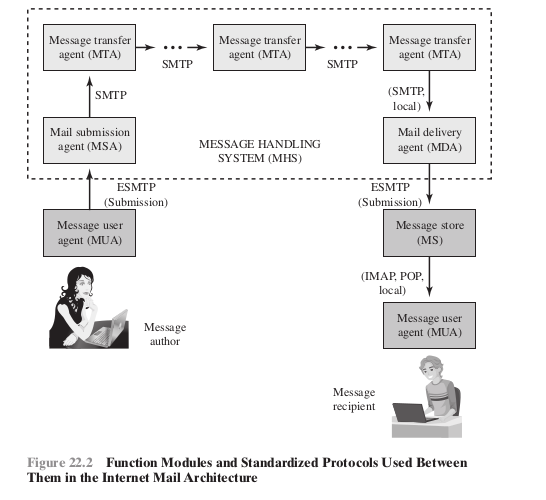
\includegraphics[width=14cm, keepaspectratio]{Bistarelli/img/cap_22/figura22.2.png}
\end{figure}

La Figura 22.2 illustra i componenti chiave dell'architettura della posta Internet, che comprendono i seguenti elementi:

\begin{itemize}
    \item \textbf{Agente utente del messaggio (MUA):} Lavora per conto degli attori utente e delle applicazioni utente. utenti e delle applicazioni degli utenti. È il loro rappresentante all'interno del servizio di posta elettronica. In genere, questa funzione è ospitata nel computer dell'utente e viene indicata come programma di posta elettronica client o server di posta elettronica della rete locale. 
    
    L'autore MUA formatta un messaggio e lo invia all'MHS tramite un programma di l'invio iniziale nel sistema MHS tramite un MSA. Il MUA destinatario elabora la posta la posta ricevuta per l'archiviazione e/o la visualizzazione all'utente destinatario.
    
    \item \textbf{Agente di invio della posta (MSA):} Accetta il messaggio inviato da un MUA e applica le politiche del dominio ospitante e i requisiti degli standard Internet.
    
    Questa funzione può essere collocata insieme al MUA o come modello funzionale separato. In quest'ultimo caso, tra il MUA e il dominio di hosting viene utilizzato il Simple Mail Transfer Protocol (SMTP).
    
    \item \textbf{Agente di trasferimento dei messaggi (MTA):} Trasmette la posta per un salto a livello di applicazione.
    
    È simile a un commutatore di pacchetti o a un router IP, in quanto il suo compito è quello di fare valutazioni di instradamento e spostare il messaggio più vicino ai destinatari. Il relay viene eseguito da una sequenza di MTA finché il messaggio non raggiunge un MDA di destinazione. Un MTA aggiunge anche aggiunge informazioni di tracciamento all'intestazione del messaggio. SMTP viene utilizzato tra gli MTA e tra un MTA e un MSA o MDA.
    
    \item \textbf{Agente di consegna della posta (MDA):} Responsabile del trasferimento del messaggio dal MHS al MS.
    
    \item \textbf{Message store (MS):} un MUA può utilizzare un MS a lungo termine. Un MS può essere un MS può trovarsi su un server remoto o sullo stesso computer del MUA. In genere, un MUA recupera i messaggi da un server remoto usando POP (Post Office Protocol) o IMAP (Internet Message Protocol).
\end{itemize}
\subsection{Strategia DKIM}
DKIM è stato progettato per fornire una tecnica di autenticazione della posta elettronica trasparente all'utente finale. In sostanza, il messaggio di posta elettronica di un utente è firmato da una chiave privata del dominio amministrativo da cui proviene l'e-mail. La firma copre tutto il contenuto del messaggio e alcune delle intestazioni del messaggio RFC 5322 (Internet Message Format, 2008). All'estremità ricevente, l'MDA può accedere alla chiave pubblica corrispondente tramite un DNS e verificare la firma, autenticando così che il messaggio proviene dal dominio amministrativo dichiarato. Pertanto, la posta che proviene da un altro luogo ma che afferma di provenire da un determinato dominio non supererà il test di autenticazione e potrà essere rifiutata. test di autenticazione e può essere rifiutata. Questo approccio differisce da quello di S/MIME, che utilizza la chiave privata dell'originatore per firmare i messaggi.

\singlespacing

La motivazione del DKIM si basa sul seguente ragionamento:

\begin{enumerate}
    \item  S/MIME dipende dall'utilizzo di S/MIME da parte degli utenti mittenti e riceventi.
    
    Per quasi tutti gli utenti, la maggior parte della posta in arrivo non utilizza S/MIME, e la maggior parte della posta che l'utente vuole ricevere non viene firmata.
    
    \item S/MIME firma solo il contenuto del messaggio. 
    
    Pertanto, le informazioni dell'intestazione RFC 5322 sull'origine possono essere compromesse.
    
    \item DKIM non è implementato nei programmi client (MUA) ed è quindi trasparente per l'utente.
    
    \item DKIM si applica a tutta la posta dei domini che collaborano.
    
    \item DKIM consente ai mittenti corretti di dimostrare di aver inviato un determinato messaggio e di impedire ai falsari di mascherarsi.
\end{enumerate}

\begin{figure}[H]
	\centering
    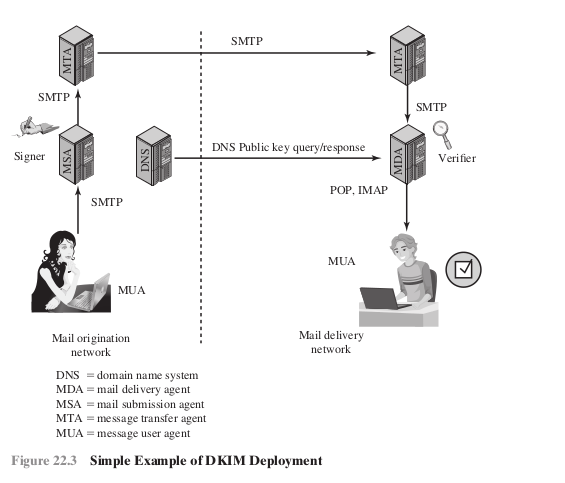
\includegraphics[width=14cm, keepaspectratio]{Bistarelli/img/cap_22/figura22.3.png}
\end{figure}

La Figura 22.3 mostra un semplice esempio del funzionamento di DKIM. Si parte da un messaggio generato da un utente e trasmesso nell'MHS a un MSA che si trova nel dominio amministrativo dell'utente. Un messaggio di posta elettronica viene generato da un programma client di posta elettronica. Il contenuto del messaggio, più le intestazioni RFC 5322 selezionate, è firmato dal provider di posta elettronica dal provider di posta elettronica utilizzando la chiave privata del provider. Il firmatario è associato a un dominio, che può essere una rete locale aziendale, un ISP o una struttura di posta elettronica pubblica come Gmail. Il messaggio firmato passa poi in Internet attraverso una sequenza di MTA. A destinazione, l'MDA recupera la chiave pubblica per la firma in arrivo e verifica la firma prima di in entrata e verifica la firma prima di passare il messaggio al client di posta elettronica di destinazione. e-mail di destinazione. L'algoritmo di firma predefinito è RSA con SHA-256. È possibile utilizzare anche RSA con SHA-1 può anche essere utilizzato.

\section{Secure Sockets Layer (SSL) e Transport Layer Security (TLS)}

Uno dei servizi di sicurezza più utilizzati è il Secure Sockets Layer (SSL) e il successivo standard Internet RFC 4346 (The Transport Layer Security (TLS) Protocol Version 1.1, 2006). TLS ha ampiamente soppiantato le precedenti implementazioni di SSL. TLS è un servizio di uso generale implementato come una serie di protocolli che si basano su TCP. A questo livello, ci sono due scelte di implementazione. Per ottenere la massima generalità, TLS potrebbe essere fornito come parte della suite di protocolli sottostante e quindi essere trasparente alle applicazioni. In alternativa, TLS può essere incorporato in pacchetti specifici. Ad esempio, la maggior parte dei browser è dotata di SSL e la maggior parte dei server Web ha implementato il protocollo.
\subsection{Architettura TLS}

\begin{figure}[H]
	\centering
    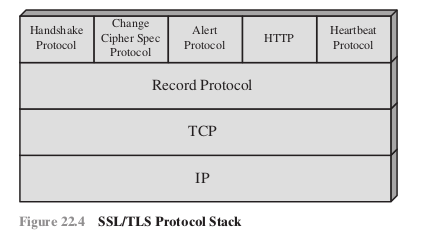
\includegraphics[width=14cm, keepaspectratio]{Bistarelli/img/cap_22/figura22.4.png}
\end{figure}

TLS è stato progettato per utilizzare il protocollo TCP e fornire un servizio sicuro end-to-end affidabile. TLS non è un singolo protocollo, ma piuttosto due livelli di protocolli, come illustrato nella Figura 22.4. Il protocollo Record fornisce servizi di sicurezza di base a vari protocolli di livello superiore. Il protocollo Record fornisce servizi di sicurezza di base a vari protocolli di livello superiore. In particolare, l'Hypertext Transfer Protocol (HTTP), che fornisce il servizio di trasferimento per l'interazione tra client e server Web, può operare su TLS. Tre protocolli di livello superiore sono definiti come parte di TLS: \textbf{il protocollo Handshake}, \textbf{il protocollo Change Cipher Spec} e \textbf{il protocollo Alert}. 

\singlespacing

Questi protocolli specifici di TLS sono utilizzati nella gestione degli scambi TLS e sono esaminati più avanti in questa sezione. Due importanti concetti di TLS sono la sessione TLS e la connessione TLS, definiti nella specifica come segue:
\begin{itemize}
    \item \textbf{Connessione:} Una connessione è un trasporto (secondo la definizione del modello di stratificazione OSI) che fornisce un tipo di servizio adeguato. Per TLS, tali connessioni sono relazioni peer-to-peer.
    
    Le connessioni sono transitorie. Ogni connessione è associata a una sessione.
    
    \item \textbf{Sessione:} Una sessione TLS è un'associazione tra un client e un server. Le sessioni sono create dal protocollo Handshake. 
    
    Le sessioni definiscono un insieme di parametri di sicurezza parametri di sicurezza, che possono essere condivisi tra più connessioni. Le sessioni sono utilizzate per evitare la costosa negoziazione di nuovi parametri di sicurezza per ogni connessione.
    
\end{itemize}
Tra qualsiasi coppia di parti (applicazioni come HTTP su client e server), possono esistere più connessioni sicure. In teoria, possono esistere anche più sessioni simultanee tra le parti, ma questa caratteristica non viene utilizzata nella pratica.
\subsection{Protocollo TLS}
Protocollo di registrazione Il protocollo di registrazione SSL fornisce due servizi per le connessioni SSL.
per le connessioni SSL:

\begin{itemize}
    \item  \textbf{Riservatezza:} Il protocollo Handshake definisce una chiave segreta condivisa che viene utilizzata per la crittografia simmetrica dei payload SSL.
    
    \item \textbf{Integrità del messaggio:} Il protocollo di handshake definisce anche una chiave segreta condivisa che viene utilizzata per formare un codice di autenticazione dei messaggi (MAC).
\end{itemize}

\begin{figure}[H]
	\centering
    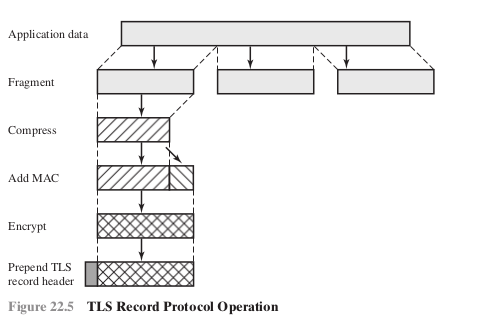
\includegraphics[width=14cm, keepaspectratio]{Bistarelli/img/cap_22/figura22.5.png}
\end{figure}

La Figura 22.5 indica il funzionamento complessivo del protocollo SSL Record. Il primo passo è la frammentazione.
Ogni messaggio di livello superiore viene frammentato in blocchi di 214 byte (16.384 byte) o meno. Successivamente, viene applicata facoltativamente la compressione. La fase successiva dell'elaborazione consiste nel calcolare un codice di autenticazione del messaggio sui dati compressi. dati compressi. Successivamente, il messaggio compresso e il MAC vengono crittografati utilizzando la crittografia simmetrica. simmetrica. L'ultima fase dell'elaborazione del protocollo SSL Record è l'aggiunta di un'intestazione, che comprende i campi di versione e lunghezza. I tipi di contenuto definiti sono change\_cipher\_spec, alert, handshake e application\_data. 

\singlespacing

I primi tre sono i protocolli specifici di TLS, di cui si parlerà in seguito.  Si noti che non viene fatta alcuna distinzione tra le varie applicazioni (ad es, HTTP) che potrebbero utilizzare TLS; il contenuto dei dati creati da tali applicazioni non è visibile a TLS. Il protocollo Record trasmette quindi l'unità risultante in un segmento TCP. I dati ricevuti vengono decifrati, verificati, decompressi e riassemblati, quindi consegnati agli utenti di livello superiore.
agli utenti di livello superiore.

\singlespacing

\paragraph{Change Cipher Spec Protocol} Il Change Cipher Spec Protocol è uno dei quattro protocolli specifici di TLS.
quattro protocolli specifici di TLS che utilizzano il TLS Record Protocol ed è il più semplice. Questo protocollo è costituito da un singolo messaggio, che consiste in un singolo byte con valore valore 1. L'unico scopo di questo messaggio è far sì che lo stato in sospeso venga copiato nello stato corrente. nello stato corrente, che aggiorna la suite di cifratura da utilizzare su questa connessione. 

\singlespacing

\paragraph{Protocollo di avviso} Il protocollo di avviso viene utilizzato per trasmettere all'entità peer avvisi relativi a TLS. Come per altre applicazioni che utilizzano TLS, i messaggi di avviso sono compressi e crittografati, come specificato e criptati, come specificato dallo stato corrente. Ogni messaggio di questo protocollo è composto da due byte. Il primo byte assume il valore\textbf{warning} o \textbf{fatal} per indicare la gravità del messaggio. Se il livello è fatale, TLS termina immediatamente la connessione. Altre connessioni sulla stessa sessione possono continuare, ma non possono essere stabilite nuove connessioni su questa sessione. Il secondo byte contiene un codice che indica l'avviso specifico. Un esempio di avviso fatale è un MAC errato. Un esempio di avviso non fatale è un messaggio close\_notify, che informa il destinatario che il mittente non invierà più messaggi su questa connessione.

\singlespacing

\paragraph{Protocollo Handshake} La parte più complessa di TLS è il protocollo Handshake. Questo protocollo consente al server e al client di autenticarsi reciprocamente e di negoziare un algoritmo di crittografia e MAC e le chiavi crittografiche da utilizzare per proteggere i dati inviati in un record TLS. Il protocollo Handshake viene utilizzato prima di trasmettere i dati dell'applicazione.

\singlespacing

\begin{figure}[H]
	\centering
    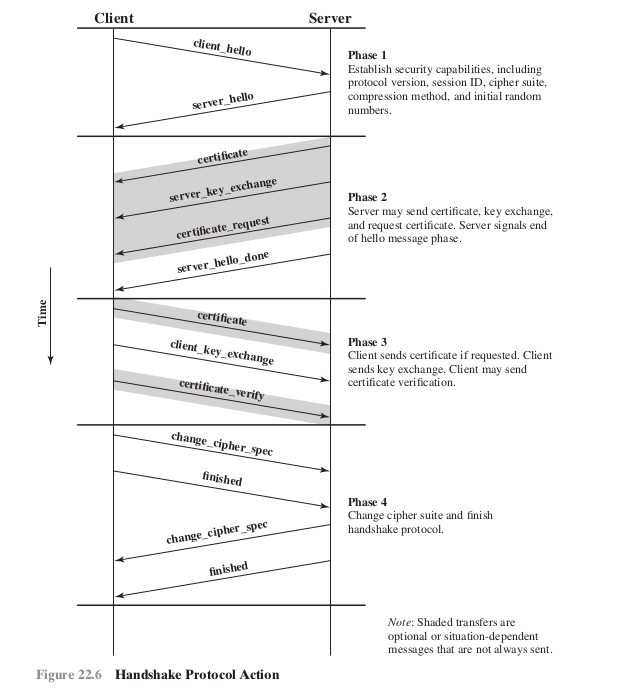
\includegraphics[width=14cm, keepaspectratio]{Bistarelli/img/cap_22/figura22.6.png}
\end{figure}

Il protocollo Handshake consiste in una serie di messaggi scambiati da client e server.

\singlespacing

La Figura 22.6 mostra lo scambio iniziale necessario per stabilire una connessione logica tra client e server. Lo scambio può essere visto come composto da quattro fasi. 

\paragraph{La fase 1} serve ad avviare una connessione logica e a stabilire le capacità di sicurezza che vi saranno associate. Lo scambio è avviato dal client, che invia un messaggio client\_hello con i seguenti parametri:

\begin{itemize}
    \item Versione: La versione TLS più alta compresa dal client.
    
    \item Casuale: Una struttura casuale generata dal client, composta da un timestamp a 32 bit e da 28 byte generati da un generatore di numeri casuali sicuri.
    
    \item ID sessione: Un identificatore di sessione di lunghezza variabile. Un valore non nullo indica che un valore non nullo indica che il client desidera aggiornare i parametri di una connessione esistente o creare una nuova connessione su questa sessione. Un valore nullo indica che il client desidera stabilire una nuova connessione in una nuova sessione.
    
    \item CipherSuite: È un elenco che contiene le combinazioni di algoritmi crittografici supportati dal client, crittografiche supportate dal client, in ordine decrescente di preferenza. Ogni elemento dell'elenco (ogni suite di cifratura) definisce sia un algoritmo di scambio di chiavi che un CipherSpec.
    
    \item Metodo di compressione: È un elenco dei metodi di compressione supportati dal client.
\end{itemize}
Dopo aver inviato il messaggio client\_hello, il client attende il messaggio server\_hello, che contiene gli stessi parametri del messaggio client\_hello.

\singlespacing

\paragraph{Fase 2} i dettagli dipendono dallo schema di crittografia a chiave pubblica utilizzato. In alcuni casi, il server passa un certificato al client, eventualmente informazioni aggiuntive sulla chiave e una richiesta di certificato da parte del client. Il messaggio finale della fase 2, che è sempre richiesto, è il messaggio server\_done, che viene inviato dal server per indicare la fine del server hello e dei messaggi associati. Dopo l'invio di questo messaggio, il server attende la risposta del client.

\singlespacing

\paragraph{Fase 3} dopo aver ricevuto il messaggio server\_done, il client deve verificare che il server abbia fornito un certificato valido se il server abbia fornito un certificato valido, se richiesto, e verificare che i parametri di server\_hello siano accettabili. Se tutto è soddisfacente, il client invia uno o più messaggi al server, a seconda dello schema a chiave pubblica sottostante.

\singlespacing

\paragraph{Fase 4} completa l'impostazione di una connessione sicura. Il client invia un messaggio messaggio change\_cipher\_spec e copia il CipherSpec in sospeso nel CipherSpec corrente. Si noti che questo messaggio non è considerato parte del protocollo di handshake, ma viene ma viene inviato utilizzando il protocollo Change Cipher Spec. Il client invia quindi immediatamente il messaggio finito con i nuovi algoritmi, chiavi e segreti. Il messaggio finito verifica che i processi di scambio di chiavi e di autenticazione siano andati a buon fine. In risposta a questi due messaggi, il server invia il proprio messaggio change\_cipher\_ spec, trasferisce il pending al CipherSpec corrente e invia il suo messaggio finito. e invia il suo messaggio finito. A questo punto, l'handshake è completo e il client e il server possono iniziare a scambiare dati di livello applicativo. 

\singlespacing

\paragraph{Protocollo Heartbeat} Nell'ambito delle reti di computer, un heartbeat è un segnale di pericolo generato dall'hardware o dal software per indicare il normale funzionamento o per indicare la presenza di un'interfaccia.
segnale peridico generato dall'hardware o dal software per indicare il normale funzionamento o per sincronizzare altre parti del sistema. Il protocollo Heartbeat si basa sul protocollo TLS Record e si compone di due tipi di messaggi: heartbeat (cuore), heartbeat (cuore) e heartbeat (cuore), due tipi di messaggi: heartbeat\_request e heartbeat\_response. L'uso del del protocollo Heartbeat viene stabilito durante la fase 1 del protocollo Handshake (vedi Figura 22.6). 

\begin{figure}[H]
	\centering
    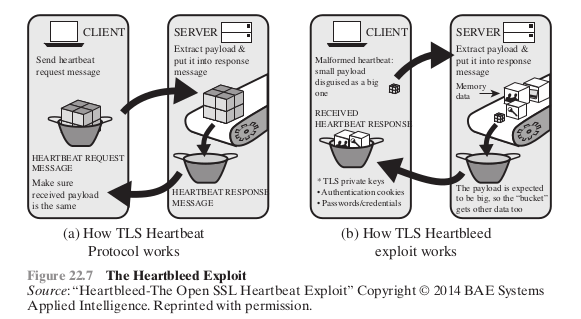
\includegraphics[width=14cm, keepaspectratio]{Bistarelli/img/cap_22/figura22.7.png}
\end{figure}

Ogni peer indica se supporta gli heartbeat. Se i battiti cardiaci sono supportati, il peer indica se è disposto a ricevere messaggi heartbeat\_request e a rispondere con messaggi heartbeat\_request. e rispondere con messaggi heartbeat\_response o se è disposto solo a inviare messaggi heartbeat\_request. Un messaggio heartbeat\_request può essere inviato in qualsiasi momento. Ogni volta che viene ricevuto un messaggio di richiesta, si deve rispondere prontamente con un corrispondente messaggio di risposta heartbeat di risposta. Il messaggio heartbeat\_request include la lunghezza del payload, il payload, e campi di riempimento. Il payload è un contenuto casuale di lunghezza compresa tra 16 byte e 64 Kbyte. di lunghezza. Il messaggio heartbeat\_response corrispondente deve includere una copia esatta del payload ricevuto. del payload ricevuto. Anche il padding è un contenuto casuale. Il padding consente al il mittente di eseguire un'operazione di scoperta dell'unità massima di trasferimento (MTU) del percorso, inviando richieste con padding crescente fino a quando non si ottiene più risposta. 

\singlespacing

Il battito cardiaco ha due scopi. In primo luogo, assicura al mittente che il destinatario è ancora vivo, anche se per un po' di tempo non c'è stata alcuna attività sulla connessione TCP sottostante. In secondo luogo, l'heartbeat genera attività sulla connessione durante i periodi di inattività, evitando così la chiusura da parte di un firewall che non tollera le connessioni inattive. Il requisito dello scambio di un carico utile è stato progettato nel sistema Heartbeat
per supportarne l'uso in una versione senza connessione di TLS, nota come DTLS. Poiché un servizio senza connessione è soggetto alla perdita di pacchetti, il carico utile consente al richiedente di abbinare i messaggi di risposta alle richieste. Per semplicità, la stessa versione del protocollo Heartbeat viene utilizzata sia con TLS che con DTLS. Pertanto, il carico utile è necessario sia per TLS che per DTLS.

\newpage

\subsection{Attacchi SSL/TLS}
Dalla prima introduzione di SSL nel 1994 e dalla successiva standardizzazione di TLS, sono stati ideati numerosi attacchi contro questi protocolli. La comparsa di ogni attacco ha reso necessarie modifiche al protocollo, agli strumenti di crittografia utilizzati o ad alcuni aspetti dell'implementazione di SSL e TLS per contrastare queste minacce.

\singlespacing

Categorie di attacchi Possiamo raggruppare gli attacchi in quattro categorie generali:

\begin{itemize}
    \item Attacchi al protocollo Handshake: Già nel 1998, un approccio al protocollo Handshake basato sul promettere il protocollo Handshake basato sullo sfruttamento della formattazione e dell'implementazione dello schema di crittografia RSA. Con l'implementazione di contromisure sono state implementate, l'attacco è stato perfezionato e adattato per non solo per vanificare le contromisure, ma anche per velocizzare l'attacco.
    
    \item Attacchi ai protocolli di registrazione e di dati applicativi: Sono state scoperte numerose vulnerabilità in questi protocolli.
    
    \item Attacchi alla PKI: la verifica della validità dei certificati X.509 è un'attività soggetta a una serie di attacchi, sia in una serie di attacchi, sia nel contesto di SSL/TLS che altrove.
\end{itemize}
\section{HTTPS}
HTTPS (HTTP over SSL) si riferisce alla combinazione di HTTP e SSL per implementare una comunicazione sicura tra un browser Web e un server Web. La funzionalità HTTPS è integrata in tutti i browser Web moderni. Il suo utilizzo dipende dal server Web che supporta la comunicazione HTTPS. La differenza principale per l'utente di un browser Web è che gli indirizzi URL (uniform resource locator) iniziano con https:// invece che con http://. Una normale connessione HTTP
utilizza la porta 80. Se viene specificato HTTPS, viene utilizzata la porta 443, che richiama SSL.

\singlespacing

Quando si utilizza HTTPS, i seguenti elementi della comunicazione sono crittografati:

\begin{itemize}
    \item URL del documento richiesto
    
    \item Contenuto del documento
    
    \item Contenuto dei moduli del browser (compilati dall'utente del browser)
    
    \item  Cookie inviati dal browser al server e dal server al browser
    
    \item  Contenuto dell'intestazione HTTP
\end{itemize}

\subsection{Avvio della connessione}
Per HTTPS, l'agente che agisce come client HTTP agisce anche come client TLS. Il client avvia una connessione al server sulla porta appropriata e invia il ClientHello TLS per iniziare l'handshake TLS. Quando l'handshake TLS è terminato, il client può avviare la prima richiesta HTTP. Tutti i dati HTTP devono essere inviati come dati dell'applicazione TLS. Quando l'handshake TLS è terminato, il client può avviare la prima richiesta HTTP. È necessario chiarire che ci sono tre livelli di consapevolezza di una connessione in HTTPS. A livello HTTP, un client HTTP richiede una connessione a un server HTTP inviando una richiesta di connessione al livello immediatamente inferiore. In genere, il livello più basso è il TCP, ma può anche essere il TLS/SSL. A livello di TLS, viene stabilita una sessione tra un client TLS e un server TLS. Questa sessione può supportare una o più connessioni in qualsiasi momento. Come abbiamo visto, una richiesta TLS per stabilire una connessione inizia con la creazione di una connessione TCP tra l'entità TCP sul lato client e l'entità TCP sul lato server. 

\subsection{Chiusura della connessione}
Un client o un server HTTP può indicare la chiusura di una connessione includendo la linea seguentein un record HTTP: \textbf{Connection: close.} Questo indica che la connessione sarà chiusa dopo la consegna di questo record.

\singlespacing

La chiusura di una connessione HTTPS richiede che TLS chiuda la connessione con l'entità peer TLS sul server, con l'entità peer TLS sul lato remoto, il che comporta la chiusura della connessione TCP sottostante.
A livello di TLS, il modo corretto per chiudere una connessione è che ciascuna parte utilizzi il protocollo di avviso TLS per inviare un avviso close\_notify. Le implementazioni TLS devon avviare uno scambio di avvisi di chiusura prima di chiudere una connessione.  Un'implementazione TLS può, dopo l'invio di un avviso di chiusura, chiudere la connessione senza attendere che il peer invii il suo avviso di chiusura, generando una "chiusura incompleta". Si noti che 
un'implementazione che fa questo può scegliere di riutilizzare la sessione. Questo dovrebbe essere fatto solo
solo quando l'applicazione sa (tipicamente attraverso il rilevamento dei limiti dei messaggi HTTP) di aver ricevuto tutti i dati del messaggio che le interessano.

\singlespacing

I client HTTP devono inoltre essere in grado di gestire una situazione in cui la connessione TCP viene terminata senza un avviso precedente di close\_notify e senza un indicatore di \textbf{Connection: close} indicator. Tale situazione potrebbe essere dovuta a un errore di programmazione del server o a un errore di comunicazione che causa l'interruzione della connessione TCP. Tuttavia, la chiusura TCP non annunciata potrebbe essere la prova di un qualche tipo di attacco.
Pertanto, il client HTTPS dovrebbe emettere una sorta di avviso di sicurezza quando ciò si verifica.

\section{Sicurezza IPv4 e IPv6 }
La comunità di Internet ha sviluppato meccanismi di sicurezza specifici per le applicazioni di sicurezza specifici per le applicazioni in diverse aree, tra cui la posta elettronica (S/MIME), il client/server (Kerberos), l'accesso al Web (SSL) e altri ancora.  Tuttavia, gli utenti hanno alcune preoccupazioni sulla sicurezza che riguardano livelli di protocollo. 

\singlespacing

Per esempio, un'azienda può gestire una rete TCP/IP privata e sicura disabilitando i collegamenti a siti non attendibili, criptando i pacchetti che lasciano la sede, e autenticando i pacchetti che vi entrano. Implementando la sicurezza a livello IP, un'organizzazione può garantire la sicurezza della rete non solo per le applicazioni che
meccanismi di sicurezza, ma anche per le molte applicazioni ignare della sicurezza.

\singlespacing

In risposta a questi problemi, l'Internet Architecture Board (IAB) ha incluso l'autenticazione e la crittografia come elementi necessari di autenticazione e crittografia come caratteristiche di sicurezza necessarie nell'IP di nuova generazione, che è stato rilasciato con il nome di IP. 
IP di prossima generazione, che è stato rilasciato con il nome di IPv6. Fortunatamente, queste funzionalità di sicurezza sono state fortunatamente, queste funzionalità di sicurezza sono state progettate per essere utilizzabili sia con l'attuale IPv4 che con il futuro IPv6. 

\singlespacing

Questo significa che i fornitori possono iniziare a offrire queste funzionalità fin da subito e molti di essi hanno già
alcuni prodotti con funzionalità IPsec.
La sicurezza a livello IP comprende tre aree funzionali:

\begin{enumerate}
    \item Autenticazione
    
    \item Confidenza 
    
    \item Gestione delle chiavi
\end{enumerate}

Il meccanismo di autenticazione assicura che un messaggio ricevuto sia stato trasmesso dalla parte identificata come sorgente nell'intestazione del pacchetto. Inoltre, questo meccanismo assicura che il pacchetto non sia stato alterato durante il transito. La funzione di confidenzialità consente ai nodi comunicanti di crittografare i messaggi per impedire l'intercettazione da parte di terzi. La funzione di gestione delle chiavi si occupa lo scambio sicuro di chiavi. La versione attuale di IPsec, nota come IPsecv3, comprende l'autenticazione e la riservatezza. La gestione delle chiavi è fornita dallo standard Internet Key Exchange, IKEv2.

\newpage
\paragraph{Applicazioni di Ipisec} IPsec offre la possibilità di proteggere le comunicazioni attraverso una LAN, una WAN privata e pubblica e Internet. 

\singlespacing

Esempi di di utilizzo sono i seguenti:

\begin{itemize}
    \item \textbf{Connettività sicura delle filiali su Internet:} Un'azienda può creare una rete privata virtuale sicura su Internet o su una WAN pubblica. In questo modo Internet e ridurre la necessità di reti private, risparmiando sui costi e sulla gestione delle reti private, risparmiando sui costi e sulle spese di gestione della rete.
    
    \item \textbf{Accesso remoto sicuro via Internet:} Un utente finale il cui sistema è dotato di sicurezza IP può effettuare una chiamata locale a un provider di servizi Internet e accedere in modo sicuro alla rete aziendale. In questo modo si riducono i costi di pedaggio di pedaggio per i dipendenti in viaggio e i telelavoratori.
    
    \item \textbf{Stabilire una connettività extranet e intranet con i partner:} IPsec può essere utilizzato per proteggere le comunicazioni con altre organizzazioni, garantendo l'autenticazione e la riservatezza e fornendo uno scambio di chiavi.
    
    \item \textbf{Migliorare la sicurezza del commercio elettronico:} Anche se alcune applicazioni per il Web e il commercio elettronico dispongono di protocolli di sicurezza integrati, l'uso di IPsec migliora tale sicurezza.
\end{itemize}
\textbf{La caratteristica principale di IPsec}, che gli consente di supportare queste diverse applicazioni, è la possibilità di criptare è che può crittografare e/o autenticare tutto il traffico a livello IP. In questo modo, tutte le
applicazioni distribuite, tra cui accesso remoto, client/server, e-mail, trasferimento di file, accesso al Web e così via, accesso al Web e così via, possono essere protette. La Figura 9.3 mostra uno scenario tipico di utilizzo di IPsec.

\singlespacing

\paragraph{Benefici di IPsec}
I vantaggi di IPsec sono i seguenti:
\begin{itemize}
    \item Quando IPsec è implementato in un firewall o in un router, fornisce una forte sicurezza che può essere applicata a tutto il traffico che attraversa il perimetro.
    
    \item IPsec in un firewall è resistente all'aggiramento se tutto il traffico proveniente dall'esterno deve utilizzare il protocollo IP e il firewall è l'unico mezzo di accesso al perimetro.
    
    \item IPsec si trova al di sotto del livello di trasporto (TCP, UDP) ed è quindi trasparente alle applicazioni.
     Non è necessario modificare il software di un sistema utente o server quando IPsec è implementato nel firewall o nel router.
     
    \item IPsec può essere trasparente per gli utenti finali. Non è necessario formare gli utenti sui meccanismi di sicurezza, di rilasciare materiale di chiave per ogni utente o di revocare il materiale di chiave quando gli utenti lasciano l'organizzazione.
     
    \item Se necessario, IPsec può garantire la sicurezza per i singoli utenti. Questo è utile per i lavoratori fuori sede e per la creazione di una sottorete virtuale sicura all'interno di un'organizzazione per le applicazioni sensibili.
\end{itemize}
\paragraph{Applicazioni di routing} oltre a supportare gli utenti finali e a proteggere i sistemi e le reti di una
reti e dei sistemi delle sedi, IPsec può svolgere un ruolo fondamentale nell'architettura di routing necessaria per l'internetworking.  

\singlespacing

I seguenti esempi di utilizzo di IPsec che può garantire che:

\begin{itemize}
    \item Un annuncio di router (un nuovo router pubblicizza la sua presenza) provenga da un router autorizzato.
router autorizzato.

    \item Un annuncio di vicinato (un router cerca di stabilire o mantenere una relazione di vicinato con un router di un altro paese).
    
    \item Un messaggio di reindirizzamento proviene dal router a cui è stato inviato il pacchetto iniziale.
    
    \item Un aggiornamento di routing non viene falsificato.
\end{itemize}
Senza queste misure di sicurezza, un avversario può interrompere le comunicazioni o deviare il traffico. I protocolli di routing, come l'Open Shortest Path First (OSPF), devono essere eseguiti in base a essere eseguiti sulla base di associazioni di sicurezza tra router definite da IPsec.

\subsection{Il campo di applicazione di IPsec}
IPsec fornisce due funzioni principali: una funzione combinata di autenticazione/crittografia chiamata Encapsulating Security Payload (ESP) e una funzione di scambio di chiavi. Per le reti private virtuali, in genere si desiderano sia l'autenticazione che la crittografia, perché è importante 

\begin{enumerate}
    \item Assicurare che gli utenti non autorizzati non penetrino nella rete privata virtuale
    
    \item Assicurare che gli intercettatori su Internet non possano leggere i messaggi inviati attraverso la rete privata virtuale
\end{enumerate}
Esiste anche una funzione di sola autenticazione, implementata mediante un'intestazione di autenticazione (AH). Poiché l'autenticazione dei messaggi è fornita da ESP, l'uso di AH è deprecato. È incluso in IPsecv3 per compatibilità con il passato, ma non dovrebbe essere utilizzato in nuove applicazioni. In questo capitolo non si parlerà di AH. La funzione di scambio di chiavi consente lo scambio manuale delle chiavi e uno schema automatizzato. 

\subsection{Security Associations}
Un concetto chiave che compare in entrambi i meccanismi di autenticazione e riservatezza per IP è l'associazione di sicurezza (SA). Un'associazione è una relazione unidirezionale tra un mittente e un destinatario che offre servizi di sicurezza al traffico trasportato su di essa. Se è necessaria una relazione tra pari, per uno scambio sicuro bidirezionale, sono necessarie due associazioni di sicurezza. di sicurezza. I servizi di sicurezza sono garantiti da una SA per l'uso di ESP.

\singlespacing

Una SA è identificata in modo univoco da tre parametri:

\begin{itemize}
    \item \textbf{Indice del parametro di sicurezza (SPI):} Una stringa di bit assegnata a questa SA e avente significato solo a livello locale. L'SPI è contenuto in un'intestazione ESP per consentire al sistema ricevente di selezionare il SA in base al quale il SA è stato inviato.
    
    \item \textbf{Indirizzo di destinazione IP:} È l'indirizzo dell'endpoint di destinazione del SA, che può essere un sistema dell'utente finale o un sistema di rete come un firewall o un router.
    
    \item \textbf{Identificatore di protocollo:} Questo campo dell'intestazione IP esterna indica se l'asso- ciazione è un protocollo AH o ESP.
\end{itemize}
Un'implementazione di IPsec include un database di associazioni di sicurezza che definisce i parametri associati a ogni SA. Un SA è caratterizzato dai seguenti parametri:

\begin{itemize}
    \item Contatore del numero di sequenza: Un valore a 32 bit usato per generare il campo Sequence Number nelle intestazioni AH o ESP.
    
    \item Overflow del contatore di sequenza: Un flag che indica se l'overflow del contatore di numeri di sequenza deve generare un evento verificabile e impedire l'ulteriore transazione di pacchetti su questa SA.
    
    \item Finestra antireplay: Utilizzata per determinare se un pacchetto AH o ESP in entrata è un replay, definendo una finestra scorrevole un replay, definendo una finestra scorrevole entro la quale il numero di sequenza deve rientrare.
    
    \item Informazioni AH: Algoritmo di autenticazione, chiavi, durata delle chiavi e parametri correlati utilizzati con AH.
    
    \item Informazioni su ESP: Algoritmo di crittografia e di autenticazione, chiavi, valori di inizializzazione, durate delle chiavi e parametri correlati.
    
    \item Durata di questa associazione di sicurezza: Un intervallo di tempo o un conteggio di byte dopo il quale una SA deve essere sostituita da una nuova SA (e da un nuovo SPI) o terminata, oltre a un'indicazione di quale di queste azioni deve avvenire.
    
    \item Modalità del protocollo IPsec: Tunnel, trasporto o wildcard (richiesto per tutte le implementazioni).
    
    \item MTU del percorso: Qualsiasi unità di trasmissione massima del percorso osservata (dimensione massima di un pacchetto che può essere trasmesso senza frammentazione) e variabili di invecchiamento.
\end{itemize}
Il meccanismo di gestione delle chiavi utilizzato per la distribuzione delle chiavi è collegato ai meccanismi di
meccanismi di autenticazione e privacy solo attraverso i parametri di sicurezza. Pertanto, l'autenticazione e la privacy sono state specificate indipendentemente da qualsiasi meccanismo di gestione delle chiavi.

\subsection{L'Encapsulating Security Payload}
Fornisce servizi di riservatezza, tra cui la riservatezza del contenuto dei messaggi e la riservatezza limitata del flusso di traffico. Come caratteristica opzionale, ESP può anche fornire un servizio di autenticazione. 

\begin{figure}[H]
	\centering
    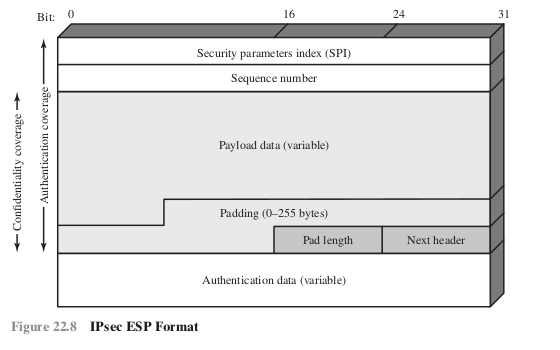
\includegraphics[width=14cm, keepaspectratio]{Bistarelli/img/cap_22/figura22.8.png}
\end{figure}

La Figura 22.8 mostra il formato di un pacchetto ESP. Esso contiene i seguenti campi:
\begin{itemize}
    \item \textbf{Indice dei parametri di sicurezza (32 bit):} Identifica un'associazione di sicurezza.
    
    \item \textbf{Numero di sequenza (32 bit):} Un valore di contatore monotonicamente crescente.
    
    \item \textbf{Dati del carico utile (variabile):} Si tratta di un segmento a livello di trasporto (modalità di trasporto) o di un pacchetto IP (modalità tunnel) protetto da crittografia.
    
    \item\textbf{Padding (0-255 byte):} Può essere necessario se l'algoritmo di crittografia richiede che il testo in chiaro sia il testo in chiaro sia un multiplo di un certo numero di ottetti.
    
    \item \textbf{Lunghezza pad (8 bit):} Indica il numero di byte di pad immediatamente precedenti a questo campo.
    
    \item \textbf{Intestazione successiva (8 bit):} Identifica il tipo di dati contenuti nel campo Dati payload identificando la prima intestazione del carico utile (ad esempio, un'intestazione di estensione in IPv6 o un'intestazione superiore).
    
    \item \textbf{Valore di controllo dell'integrità (variabile):} Un campo di lunghezza variabile (deve essere un numero integrale di parole a 32 bit) che contiene il valore di controllo dell'integrità calcolato su il pacchetto ESP meno il campo Dati di autenticazione.
\end{itemize}

\subsection{Transport and Tunnel Modes}
L'ESP supporta due modalità di utilizzo: quella di trasporto e quella di tunnel. Iniziamo questa sezione con una breve panoramica.

\paragraph{Modalità di trasporto} La modalità di trasporto fornisce protezione principalmente ai protocolli di livello superiore. In altre parole, la protezione in modalità trasporto si estende al carico utile di un pacchetto IP. Tra gli esempi vi sono i segmenti TCP o UDP, che operano entrambi direttamente sopra l'IP nello stack di protocolli dell'host. In genere, la modalità di trasporto viene utilizzata per la comunicazione end-to-end tra due host (ad esempio, un client e un server o due workstation). Quando un host esegue ESP su IPv4, il payload è costituito dai dati che normalmente seguono l'intestazione IP. Per IPv6, il payload è costituito dai dati che normalmente seguono l'intestazione IP e le eventuali intestazioni di estensione IPv6 presenti, con l'eventuale eccezione dell'intestazione delle opzioni di destinazione di destinazione, che può essere inclusa nella protezione. ESP in modalità di trasporto cripta e, facoltativamente, autentica il payload IP, ma non l'intestazione IP. 

\singlespacing

\paragraph{Modalità tunnel} La modalità tunnel fornisce protezione all'intero pacchetto IP. Per ottenere
Per ottenere questo risultato, dopo che i campi ESP sono stati aggiunti al pacchetto IP, l'intero pacchetto più i campi 
di sicurezza viene trattato come il carico utile di un nuovo pacchetto IP esterno con una nuova intestazione IP esterna.
L'intero pacchetto originale, interno, viaggia attraverso un tunnel da un punto all'altro di una rete IP.
da un punto all'altro di una rete IP; nessun router lungo il percorso è in grado di esaminare l'intestazione IP interna.
Poiché il pacchetto originale è incapsulato, il nuovo pacchetto più grande può avere indirizzi di origine e di destinazione completamente diversi, il che aumenta la sicurezza. La modalità tunnel viene utilizzata quando una o entrambe le estremità di un'associazione di sicurezza sono un gateway di sicurezza, come un firewall o un router che implementa IPsec. Con la modalità tunnel, un certo numero di host su reti dietro firewall può effettuare comunicazioni sicure senza implementare IPsec. I pacchetti non protetti generati da tali host vengono inoltrati attraverso le reti reti esterne tramite SA in modalità tunnel impostati dal software IPsec nel firewall o nel router sicuro al confine del o router sicuro al confine della rete locale. 

\singlespacing

\textbf{Ecco un esempio di come funziona IPsec in modalità tunnel.}

\singlespacing

L'host A su una rete genera un pacchetto IP con l'indirizzo di destinazione dell'host B su un'altra rete, simile a quello mostrato nella Figura 9.3. Questo pacchetto viene instradato dall'host di origine verso un firewall o un router sicuro a un firewall o a un router sicuro al confine della rete di A. Il firewall filtra tutti i pacchetti IP con l'indirizzo di destinazione dell'host B. Il firewall filtra tutti i in uscita per determinare la necessità di un'elaborazione IPsec. Se questo pacchetto da A a B richiede IPsec, il firewall esegue l'elaborazione IPsec e incapsula il pacchetto con un'intestazione IP esterna. pacchetto con un'intestazione IP esterna. L'indirizzo IP di origine di questo pacchetto IP esterno è questo firewall, mentre l'indirizzo di destinazione può essere un firewall che delimita la rete locale di B. rete locale di B. Il pacchetto viene ora instradato verso il firewall di B, con router intermedi che esaminano solo l'intestazione IP esterna. esaminano solo l'intestazione IP esterna. Al firewall di B, l'intestazione IP esterna viene eliminata e il pacchetto interno viene e il pacchetto interno viene consegnato a B. L'ESP in modalità tunnel cripta e, facoltativamente, autentica l'intero pacchetto IP interno, compresa l'intestazione IP interna.

